\section{Experimental methods}
\label{sec:dbb:exp}

\subsection{Materials}

The batteries used in this study are Duracell MN1500 Coppertop LR6 batteries with a nominal initial voltage of 1.65 V, and a nominal capacity of 2850 mAh. Prior to testing, a representative LR6 cell is dismantled and the individual parts weighed to determine component mass. Weighing is performed using a Metler-Toledo lab balance accurate to 0.1 mg. Components are then dried at 25°C under vacuum for 48 hours in a VWR Symphony vacuum oven, after which components are again weighed to determine system mass after dehydration.

Batteries are discharged at a rate of roughly C/10 (280 mA) using a Neware BT3000-8 cycler for one hour intervals followed by a 15 minute rest period at open-circuit conditions, prior to performing electrochemical impedance spectroscopy and drop testing. Following every discharge cycle, batteries are weighed to determine whether mass loss had occurred during discharge.


\subsection{Electrochemical impedance spectroscopy}

Electrochemical impedance spectroscopy is performed on each cell using a Gamry Reference 3000 unit after every 280 mAh of capacity discharge. Scans are performed under potentiostatic conditions at the open circuit voltage of each cell, with an AC voltage perturbation of 10 mV, sweeping from 100 mHz to 100 kHz. 



\subsection{Bounce tests}

Batteries are dropped 25 cm through an acrylic tube of 18 mm diameter onto an epoxy bench top, as shown in the schematic in Fig.~\ref{fig:expschem}. 

\begin{figure}[htb]
  \centering
    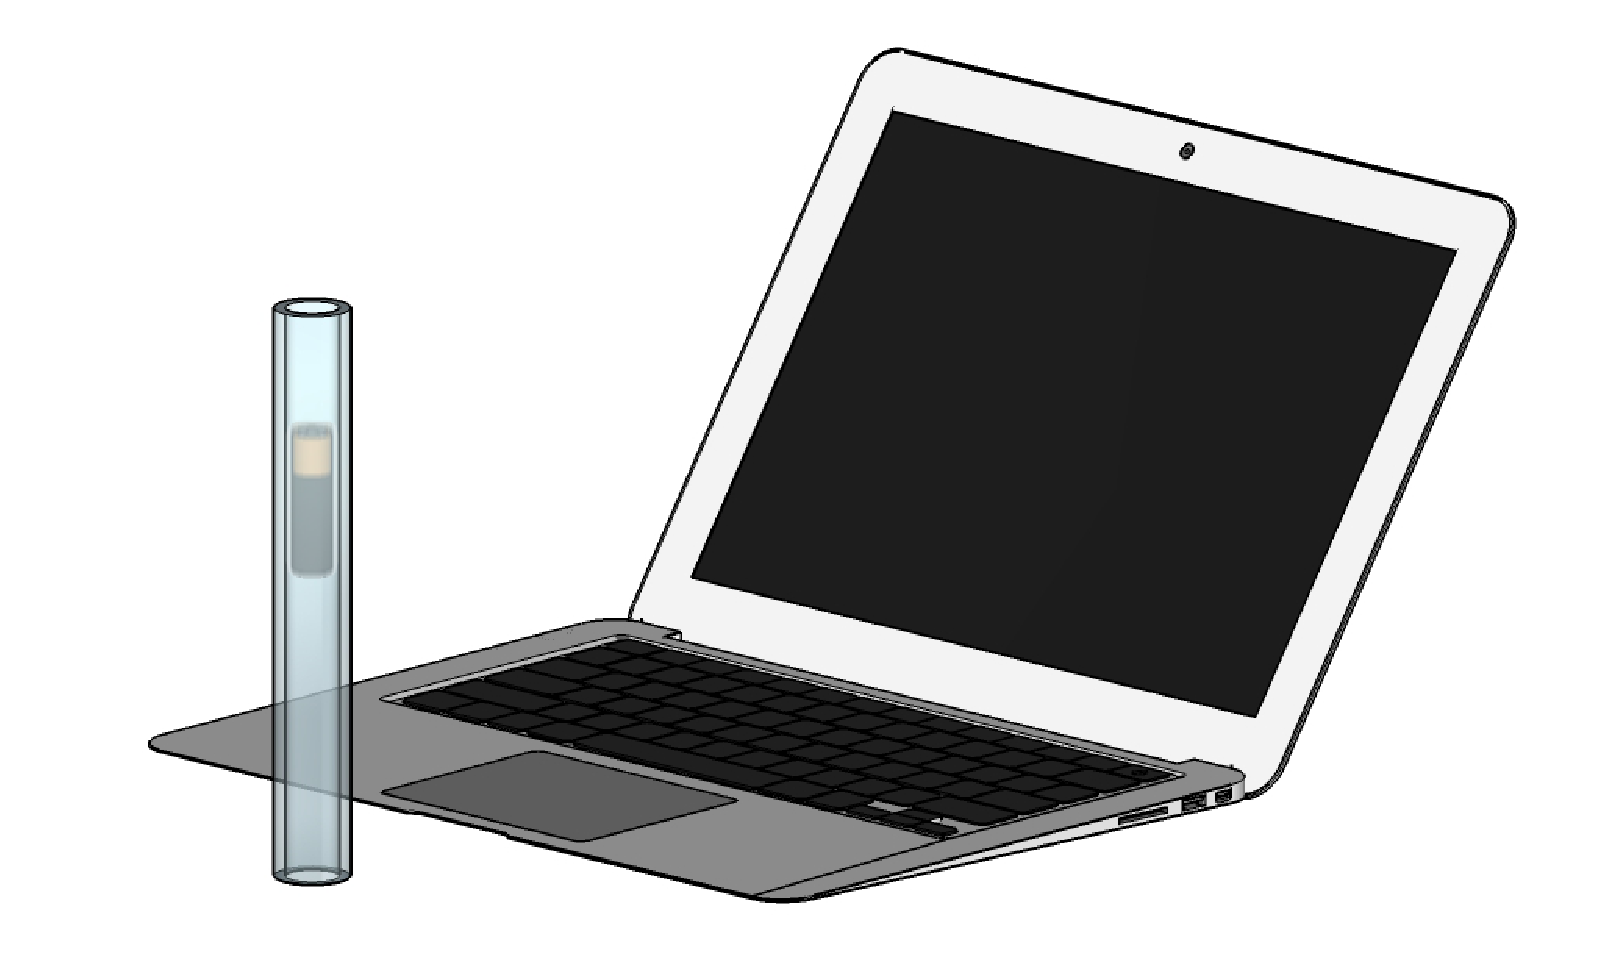
\includegraphics[width=0.75\textwidth]{ch3-dbb/Images/Setup.eps}
    \caption[Schematic of bounce test experiments.]{Schematic of construction of bounce test experiments.}
    \label{fig:expschem}
\end{figure}

The usage of the acrylic tube ensures equivalence of each drop test. The audio profile of each drop is recorded using a microphone placed 30 cm away, and later analyzed using a python script to determine number of bounces, height of bounce, and coefficient of restitution. The height of each bounce was determined by the relationship

\begin{equation}
h_{bounce}= \frac{1}{2}g(\frac{\Delta t_{bounce}}{2})^2
\label{eq:bounce}
\end{equation}

\noindent where {\ce{\Delta t_{bounce}}} is the time measured between bounces with the microphone.

\subsection{Energy dispersive x-ray diffraction}

\textit{In situ} energy dispersive XRD was performed at Beamline X17B1 of the National Synchrotron Light Sources (NSLS) at Brookhaven National Laboratory.  Beamline X17B1 is an energy dispersive x-ray line capable of measuring internal structural changes in a discrete volume. LR6 batteries were analyzed using methodology that has been described in detail by Gallaway et al.~\cite{gallaway}